\icode[magenta]{N22Q-MI-SI-L4-261108-002}
\nceeID[unkown]{2022海南卷}{8}
我国的石桥世界闻名，如图，某桥由六块形状完全相同的石块组成，其中石块1、6固定，2、5质量相同为\(m\)，3、4质量相同为\(m^{\prime}\)，不计石块间的摩擦，则\(m:m^{\prime}\)为\paren[]

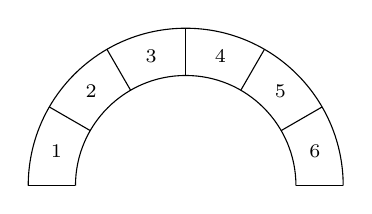
\begin{tikzpicture}[font=\scriptsize]
	\foreach \d in {0,30,...,180}
		\draw (\d:1.4)--(\d:2);
	\draw (0:1.4) arc(0:180:1.4);
	\draw (0:2) arc(0:180:2);
	\foreach \d/\n in {15/6,45/5,75/4,105/3,135/2,165/1}
		\node at(\d:1.7){\(\n\)};
\end{tikzpicture}
\begin{choices}
	\item\(\dfrac{\sqrt{3}}{2}\)
	\item\(\sqrt{3}\)
	\item\(1\)
	\item\(2\)
\end{choices}
\begin{answer}
	D\qquad 提示：分解力，合成力。
\end{answer}
